% vim:set et fenc=utf-8 ft=tex sw=2 ts=4 tw=84:

\newif\ifdraft
\drafttrue

\ifdraft
        \documentclass[conference, draftclsnofoot, draft]{IEEEtran}
        \def\baselinestretch{1}
        \setlength{\marginparwidth}{2cm}
\else
        \documentclass[conference]{IEEEtran}
\fi

\usepackage[T1]{fontenc}
\usepackage[utf8]{inputenc}

\usepackage[hyphens]{url} \urlstyle{same}

%% Citations
\usepackage[nospace]{cite}

%% Table Support

\usepackage{dcolumn}
\usepackage{longtable}
\usepackage{multirow}


%% Extra support
\usepackage{xspace}
\usepackage{amsmath}
\usepackage{algorithm}
\usepackage{balance}
\usepackage{placeins}


%% Graphics

\usepackage{tikz}
\usepackage{pgfplots}
\usepackage{pgfplotstable}
\usepackage{xcolor}
\usepackage{color}

%% Tikz
\usetikzlibrary{positioning, arrows}

% Chart Colors
\definecolor{chartblue}{HTML}{3366CC}
\definecolor{chartred}{HTML}{DC3912}
\definecolor{chartyellow}{HTML}{FF9900}
\definecolor{chartgreen}{HTML}{109618}
\definecolor{chartmagenta}{HTML}{990099}
\definecolor{chartpurple}{HTML}{3B3EAC}

% \ifdraft
%     \usepackage[colorinlistoftodos]{todonotes}
%     \newcommand{\evan}[1]{{\color{blue}\emph{Evan Says: #1}}\xspace}
%     \newcommand{\evantodo}[1]{{\color{blue}\emph{Evan Todo: #1}}\xspace}
%     \newcommand{\dmg}[1]{{\color{blue}\emph{dmg Says: #1}}\xspace}
%     \newcommand{\dmgtodo}[1]{{\color{blue}\emph{dmg Todo: #1}}\xspace}
% \else
%     \usepackage[disable]{todonotes}
%     \newcommand{\evan}[1]{}
%     \newcommand{\evantodo}[1]{}
%     \newcommand{\dmg}[1]{}
%     \newcommand{\dmgtodo}[1]{}
% \fi
    \usepackage[colorinlistoftodos]{todonotes}

\newcommand{\tool}{{\emph Linvis}\xspace}


    \newcommand{\evan}[1]{{\color{blue}\emph{Evan Says: #1}}\xspace}
    \newcommand{\evantodo}[1]{{\color{blue}\emph{Evan Todo: #1}}\xspace}
    \newcommand{\dmg}[1]{{\color{blue}\emph{dmg Says: #1}}\xspace}
    \newcommand{\dmgtodo}[1]{{\color{blue}\emph{dmg Todo: #1}}\xspace}


%%% Local Variables:
%%% mode: plain-tex
%%% TeX-master: t
%%% End:


\newcommand{\TheTitle}{An Evaluation and Generalization of Merge-Tree}
\newcommand{\TheAuthors}{Evan Wilde, Daniel M. German}
\newcommand{\TheEmails}{etcwilde@uvic.ca, dmg@uvic.ca}
\newcommand{\TheSubject}{Testing the comprehension of users in large git repositories}
\newcommand{\TheKeywords}{Linux, git, data structures}

\synctex=1

\begin{document}

\title{\TheTitle}

\author{
        \IEEEauthorblockA{\TheAuthors}
        \IEEEauthorblockN{Department of Computer Science,
                University of Victoria, Canada.}
        \IEEEauthorblockA{Email: \TheEmails}
}
\maketitle

\begin{abstract}

  % vim:set et sw=2 ts=4 tw=72:
With an average of more than 900 top-level merges into the Linux kernel
per release, many containing hundreds of commits and some containing
thousands, maintenance of older versions of the kernel becomes nearly
impossible.  Various commercial products, such as the Android platform,
run older versions of the kernel. Due to security, performance, and
changing hardware needs, maintainers must understand what changes
(commits) are added to the current version of the kernel since the last
time they inspected it in order to make the necessary patches.

Current tools provide information about repositories through the
directed acyclic graph (DAG) of the repository, which is helpful for
smaller projects. However, with the scale and number of branches in the
kernel the DAG becomes overwhelming very quickly. Furthermore, the DAG
contains every ancestor of every commit, while maintainers are more
interested in how and when a commit arrives to the official Linux
repository.

In this paper, we propose the merge-tree, a simplified transformation of
the DAG of the Linux git repository that shows the way in which commits
are merged into the master branch of Linux. Using the merge-tree, we
build \tool, a tool that is designed to allow users to explore how
commits are merged into the Linux kernel.

\dmg{add to the abstract the user study}

%%% Local Variables:
%%% mode: latex
%%% TeX-master: "lineval.tex"
%%% End:


\end{abstract}

\section{Introduction}
\label{sec:introduction}

% vim:set et sts=2 sw=2 ts=2 tw=72:

Between 50k and 70k commits are added to the Linux kernel per version,
requiring maintainers of older versions of the kernel to sift through
thousands of commits and merges with tools that are unable to filter and
effectively visualize projects at the scale of the kernel. Older
versions of the kernel are used in embedded systems and mobile phones;
for security purposes, performance needs, and changing hardware
requirements, maintainers must be able to understand the changes being
made in the current version of the kernel in order to produce the
necessary patches for the older versions of the kernel. Tools like Gitk
use a directed acyclic graph (DAG) model of the repository, showing all
commits and merges in chronological order by when the commit was
authored, not by when it arrived in the official Linux repository.

\begin{figure}
        \centering
        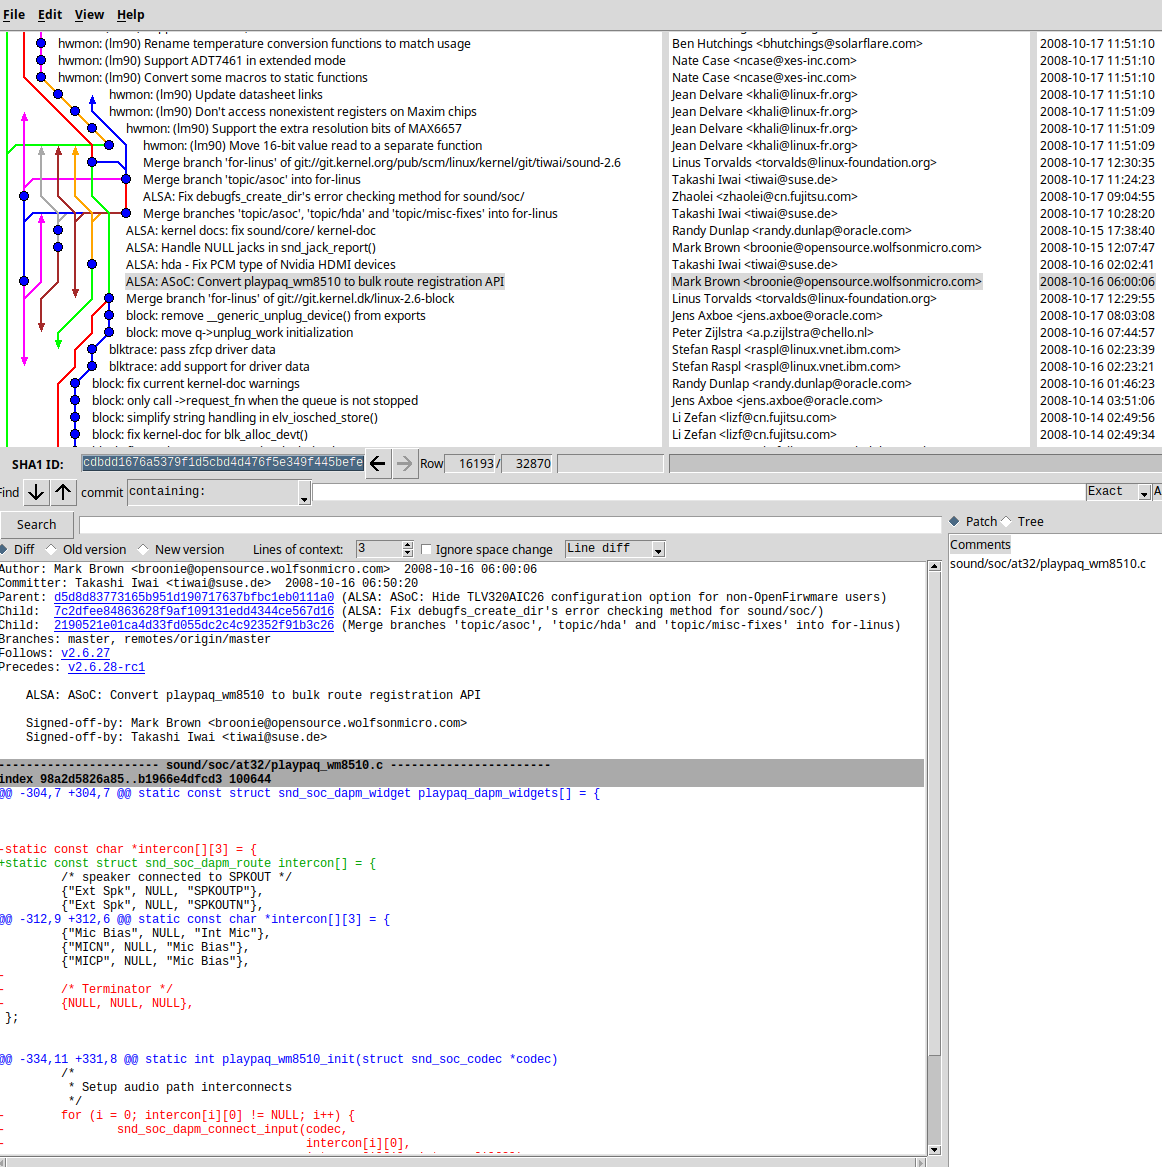
\includegraphics[width=0.97\linewidth]{figures/gitk.png}
        \caption{The Gitk interface centered on commit
          cdbdd1676a5379f1d5cbd4d476f5e349f445befe, \comB from the user
          study. The top-left pane shows the DAG and commit log preview,
          the top center pane shows the authors, and the top-right
          pane shows the commit dates. The bottom-left pane shows the
          full commit message, the parents and children of the commit,
          and the changes made to files in this commit. The bottom-right
          pane shows the list of the files modified by this commit.}
        \label{fig:gitk}
%\vspace{-4mm}
\end{figure}

\begin{figure}
        \centering
        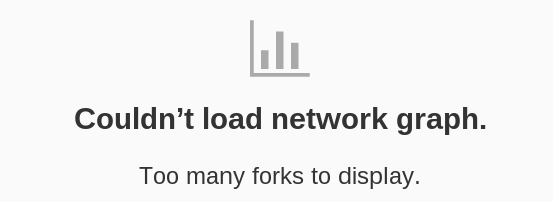
\includegraphics[width=0.8\linewidth]{figures/github_viewer.png}
        \caption{Github normally shows a visualization of the DAG,
          showing the commits, branches, and forks, but is unable to
          generate a visualization for projects at the size of the Linux
          repository.}
        \label{fig:gitfail}
%\vspace{-2mm}
\end{figure}

The DAG is able to provide a meaningful visualization in smaller
projects; it enables users to see when changes are made, when these
changes are merged, how each branch is interacting, and the point where
a branch forks from the master branch. In large modular projects, like
the Linux kernel, the DAG becomes a mess of merges and commits
(Figure~\ref{fig:gitk}) losing its visual meaning. In some cases, the
Linux kernel is simply too large for the system to generate a
visualization; Github provides a DAG view for many projects, but is
unable to display the visualization for projects at the scale of the
Linux of the kernel (Figure~\ref{fig:gitfail}). Between 60k and 70k new
commits are created for the Linux project every year; according to
previous work\cite{German2015}, a commit takes a median of 30 days from
the time it is authored until it arrives in the official repository. The
snapshot of the kernel tomorrow may be different than the snapshot from
today, containing new commits authored in the past; distinguishing these
new commits from the commits in the snapshot from today is not trivial.

One major challenge with visualizing the arrival of commits to a
repository is that Git does not store the date that a commit was merged
into another branch, including the master branch. To complicate the
problem, the DAG only has references to the ancestors of a commit (a
model necessary for the operation of Git), but maintainers would prefer
knowing the path a commit followed to reach the master repository.
Tracing a path that any commit followed to the master repository would
imply that for any given merge, it would be possible to know which
commits were merged. A user could inspect the commits that arrived into
the master branch within a given time-frame by checking which commits
were merged during that time-frame.

This paper makes three contributions; first, we describe a method of
converting the DAG of the Linux repository into the \mt of the
repository, that represents the path used by a commit to reach the
master branch; second, we present an implementation enabling the
inspection and visualization of merges in the Linux project using the
\mt modle; finally, we validate the \mt model and the implementation of
the visulization through a controlled user study. We further discuss the
issues of generalizing the model to other repositories, but present an
updated version that improves the performance of the algorithm by
pruning the DAG.\@

These methods and visualizations are implemented in a web-based tool
called \tool\footnote{\tool is currently available at
  \url{http://li.turingmachine.org}}. Our visualizations and tool
provide information about the location of any given commit or merge in
its respective merge-tree, the files edited, the modules edited, and the
commit message. \tool allows users to apply various filters, including
the release version, along with a keyword or phrase from the log
preview, the name of the author, or the commit hash. The user can
request all merges made by Linus that contain a commit or inner merge
that matches the search query, or just the commits and merges that match
the query.


\section{Related Works}
\label{sec:related_works}

\section{User Study}
\label{sec:user_study}

\dmg{start by describing what you mean by user study... to evaluate linvis we performed a user study...}

\dmg{and you are evaluating the visualizations, NOT the DAG}


We conducted a user study of \evantodo{NUMBER} participants to determine if
there is a statistically significant difference among users in
performing certain tasks on repositories between \textit{Linvis} and
either gitk or the command-line git interface. We were looking for
improvements in accuracy, time performance, and overall enjoyment among
users when performing summarization and intra-tree navigation, as these
are the tasks that merge-trees are design to simplify.

\evan{still need to figure out who our intended user is... ``git user''
  is a bit too broad.}

% TODO: Determine who the intended user is. "generic git user" is kind of broad.
% TODO: Add a note stating that we will refer to the primary branch as being the master branch

\subsubsection{Methodology}
\label{ssub:methodology}

\subsubsection{Commit Selection}
\label{ssub:commit_selection}

We selected two commits for the participant to draw and summarize by
first determining the size of tree in the first and second quartiles. We
found that between Linux 3.1 and 3.16, the size of the trees in the
first quartile only contained a single node, and that the size of the
trees in the second quartile resulted in trees up to seven nodes. The
third quartile contained trees up to 51 nodes, and the fourth quartile
contained one tree of 7217 nodes. It is worth mentioning that the tree
sizes in the fourth quartile increase very quickly, as the next largest
tree only contains 4708 nodes, and the third largest tree contains 2349
commits. We see in figure~\ref{fig:tree_size} how the number of trees
decreases as the size of the tree increases. The results for the other
plots become very noisy, since there is only one occurrence for any tree
with more than 947 commits, and only two occurrences of any trees with
size greater than 336. Due to the noise,
figures~\ref{fig:tree_size_filter},~\ref{fig:merge_count_filter},
and~\ref{fig:percentage_filter} are only on the sizes of trees where
there were at least three occurrences of trees of that size.

\pgfplotstableread[col sep=comma]{data/comdate_merge_size.csv}\comtable

\begin{figure}[htpb]
  \centering
  \begin{tikzpicture}
    \begin{axis} [
      ylabel=Tree size,
      xlabel=Date,
      grid=both
      ]
      \addplot[chartpurple] table[x index=1, y index=2]\comtable;
    \end{axis}
  \end{tikzpicture}

  \caption{Merge-tree size by date}
  \label{fig:}
\end{figure}

\pgfplotstableread[col sep=comma]{data/merge_counts.csv}\mergetable

\begin{figure}
  \centering
  \begin{tikzpicture}
    \begin{axis}[
      ylabel=Occurences,
      xlabel=Total Commits,
      grid=both,
      minor x tick num = 1,
      minor y tick num = 1
      ]
      \addplot[chartblue] table[col sep=comma, x index=1, y index=0]{data/tree_size.csv};
    \end{axis}
  \end{tikzpicture}
  \caption{Frequency of trees of varying sizes}
  \label{fig:tree_size}
\end{figure}

\begin{figure}
  \centering
  \begin{tikzpicture}
    \begin{axis}[
      ylabel=Occurences,
      xlabel=Total Commits,
      grid=both,
      minor x tick num = 1,
      minor y tick num = 1
      ]
      \addplot[chartblue] table[x index=0, y index=1]\mergetable;
    \end{axis}
  \end{tikzpicture}
  \caption{Frequency of trees of varying sizes}
  \label{fig:tree_size_filter}
\end{figure}

\begin{figure}[htpb]
  \centering
  \begin{tikzpicture}
    \begin{axis} [
      ylabel=Merges,
      xlabel=Total Commits,
      minor x tick num = 1,
      minor y tick num = 1,
      grid=both,
      legend pos = north west
      ]
      \addplot[chartred] table[x index=0, y index=5]\mergetable;
      \addlegendentry{Maximum}
      \addplot[chartyellow] table[x index=0, y index=6]\mergetable;
      \addlegendentry{Mean}
      \addplot[chartgreen] table[x index=0, y index=4]\mergetable;
      \addlegendentry{Median}
      \addplot[chartblue] table[x index=0, y index=3]\mergetable;
      \addlegendentry{Minimum}
    \end{axis}
  \end{tikzpicture}
  \caption{Number of merges versus the size of the merge tree}
  \label{fig:merge_count_filter}
\end{figure}

\begin{figure}[htpb]
  \centering
  \begin{tikzpicture}
    \begin{axis} [
      ylabel=Merge Percentage,
      xlabel=Total Commits,
      grid=both
      ]
      \addplot[chartpurple] table[x index=0, y index=7]\mergetable;
    \end{axis}
  \end{tikzpicture}
  \caption{Percentage of commits in a merge-tree that are merge commits}
  \label{fig:percentage_filter}
\end{figure}

As 25\% of the trees consist of a single commit, we selected one tree
consisting of a single commit for the study. 50\% of the trees contained
up to seven nodes, so we selected another tree of size seven.  Of these
trees, we restricted the selection to trees consisting of at least one
merge, not including the merge into the master branch.

From the list of trees consisting of a single node, we selected one at
random using the \verb|random.choice()| function in python 3.6.1, which
returned the merge tree rooted at
\emph{11df5864075f763ec0d1fdecd6a3f0af7d09a553}. As we are not testing
the inter-tree and tree-search capabilities of \emph{Linvis}, we start
the user at the corresponding commit. In this case, there is only a
single option, commit \emph{a3c1239eb59c0a907f8be5587d42e950f44543f8},
shown in Figure~\ref{fig:commit_1}.

\begin{figure}[htpb]
  \centering
  
\includegraphics[width=0.2\linewidth]{figures/commits/1-commit.pdf}
  \caption{The first merge tree used in the user study, a merge tree
    containing a single commit}
  \label{fig:commit_1}
\end{figure}

Using the same merge selection technique, we selected the tree rooted at
\emph{8eb88c80d444fd249edaa7d895666cde79e7b3b8}. To select the starting
commit, we use the python random choice function on the list of commit
hashes contained in this tree. This resulted in the selection of commit
\emph{cdbdd1676a5379f1d5cbd4d476f5e349f445befe}, shown in
Figure~\ref{fig:commit_2}.

\begin{figure}[htpb]
  \centering
  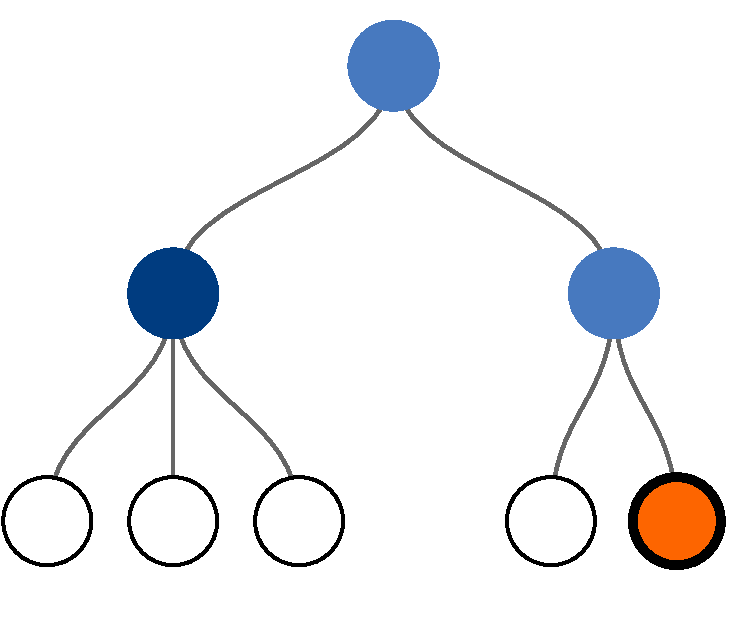
\includegraphics[width=0.5\linewidth]{figures/commits/7-commits.pdf}
  \caption{The second merge tree used in the user study, a merge tree
    containing seven commits}
  \label{fig:commit_2}
\end{figure}

\subsubsection{Questions}
\label{ssub:questions}

We chose questions that were designed to test the two primary goals of
merge trees, compared with the results from gitk or command line git.

The primary study questions are broken into two sections, one for
tree comprehension, and another section for summarization. A final
section is added, in order to have some information behind the
demographic of the participant.

\textbf{Conceptual Tasks}

As this information is provided directly by the \emph{Linvis} tree
visualizations, we use Gitk or git commandline for performing these
tasks.

\evan{Draw both trees, or just one tree?}
\begin{enumerate}
  \item Draw a diagram of the merge tree showing how the commit
    cdbdd1676a5379f1d5cbd4d476f5e349f445befe is merged into the master
    branch of the repository.
  \item How many individual commits are related to this commit?
  \item How many merges are involved with merging these commits into the
    master branch?
\end{enumerate}

We provide the user with 15 minutes to complete the first task, which is
to draw the diagram shown in Figure~\ref{fig:commit_2}. The other parts
of this task can be derived directly from the image drawn from the first
task. For this reason, we keep the ordering of these tasks consistent
between participants.

\textbf{Summarization Tasks}

We randomize the order of tool use, choosing to start with either
\emph{Linvis} or Gitk to ensure that information cannot be carried
forward from the previous tool across all participants.

The questions in this portion of the study are shuffled and presented in
random order, except where one task follows from another. We use the
\verb|random.shuffle()| function from python 3.6.1 for performing the
shuffling and presentation of the tasks.

We asked the following questions in randomized order
\begin{enumerate}
  \item What other commits are merged in the same merge
  \item What is the series of merges involved with merging this commit
  \item \label{it:aut1} How many authors are involved with this merge
  \item \label{it:aut2}Who contributed the most changes to this merge
  \item \label{it:f1}How many files were modified in this merge?
  \item \label{it:f2}Which files had the most changes in this merge?
  \item Which modules does this merge tree involve?
\end{enumerate}

We identify items \ref{it:aut1} and \ref{it:aut2} to be related,
concerning the authorship, and items \ref{it:f1} and \ref{it:f2} to be
related, concerning the files of a merge tree. The related items will be
in the same order consistently between participants, but the order of
tasks will be changed between participants.

\textbf{User Demographic}

This section of the study provides us with some information about our
participant, and how they felt about using gitk versus \emph{Linvis}.

We asked the following questions in this order
\begin{enumerate}
  \item Given these tasks again, which tool would you prefer to use?
  \item Which aspects of each tool did you like and why?
  \item How long have you used git?
  \item If you have used git, for what kind of projects? (personal,
    school courses, professional?)
  \item If you have used git, how many commits, files, and contributors
    were involved with the largest repository you have worked with?
\end{enumerate}

These questions will provide us with some information about how the user
felt, and their experience with git.

\subsubsection{Study}
\label{ssub:study}

The null hypothesis is that using merge trees or using the DAG directly
does not affect the performance of users.

%%% Local Variables:
%%% mode: latex
%%% TeX-master: t
%%% End:


\section{Generalization}
\label{sec:generalization}

The original algorithm uses a stack-like approach, which results in a depth-first
search of the tree. In the first pass, all of the commits that are in the
fist-parent position of the previous commit will be analyzed. Then following the
depth-first tactic, the tree that was earliest in the history of the repository will
be constructed, followed by the next earliest. This will be repeated until all of
the trees have been constructed and we reach the head of the master branch.

\evan{Provide a description of the new algorithm, and an DAG, and finally the
  resulting merge tree.}



\section{Discussion}
\label{sec:discussion}

\subsection{Future Work}
\label{sub:future_work}

% Inter Navigation
% TODO: verify this with the study
While the merge-tree model provides users with a better conceptual image
of what is occuring within a single merge tree, we have not exprimented
or tested the potential gains of navigation between trees. At this time,
the Linvis search provides results grouped by merge-tree root instead of
as a single block of results. The results are generally similar, with
each merge tree being merged at a different point in time, or to a
different version of the kernel. A future extension of this may
incorporate some information about how a given cluster changes over
time. To do this, a technique would need to be developed to cluster
merge-trees into modules, and then ordering the merge-trees based on
time or release.

% TODO: ensure that linvis has been referenced/defined


\section{Conclusion}
\label{sec:conclusion}

\nocite{*}

\bibliographystyle{IEEEtran}
\bibliography{references}

\end{document}
